\documentclass[a4paper]{article}
\usepackage{graphicx}
\usepackage{xcolor}
\usepackage{url}
\usepackage{outlines}
\usepackage{listings}
\lstset{basicstyle=\ttfamily,
	showstringspaces=false,
	commentstyle=\color{blue},
	keywordstyle=\color{pink}
}
\lstset{emph={
	nc,},emphstyle=\color{purple}
}
\usepackage{fancyhdr}
\usepackage{geometry}
\geometry{
	a4paper,
	total={170mm,257mm},
	left=20mm,
	top=20mm,
	bottom=39mm,
}

\setlength{\headheight}{82.70538pt}

\fancypagestyle{oida}{
	\fancyhf{}
	\fancyhead[L]{\fontsize{7.5}{7.5}htl donaustadt\\ Donaustadtstraße 45\\
		1220 Wien\\~\\ Abteilung: Informationstechnologie\\ 
	Schwerpunkt: Netzwerktechnik}
	\fancyhead[R]{
\includegraphics[scale=0.45]{images/logo.png}}

	\fancyfoot[L]{\today}
	\fancyfoot[C]{\jobname}
	\fancyfoot[R]{Seite: \thepage}
}

\begin{document}
\bibliographystyle{plain}
\pagestyle{oida}
\section*{Thema}
\par\noindent\rule{\textwidth}{0.4pt}

Laborprotokoll
TCP-UPD Header Verleich

\begin{figure}[h]
	
\includegraphics[scale=0.6]{images/meme.jpeg}
	\caption{memes klauen ist nicht ethisch}
\end{figure}

\vspace*{\fill}
Unterrichtsgegenstand:	NWT1|ZIVK

Jahrgang:	2BHIT

Name:	Stefan Fürst, Marcel Raichle

Betreuer: 	ZIVK

Übungsdaten:	24.5.2024, 31.5.2024

Abgabedatum:	Datum


\newpage
\tableofcontents

\newpage

\section{Aufgabenstellung}
TCP-UDP Header vergleich.
\section{Zusammenfassung}
Netcad um einen TCP/UPD Server starten, mit Netcad verbinden und mit Wireshark die Verbindungen analysieren.
test


\newpage

\section{Übungsdurchführung}

\subsection{Aufsetzen der Server}
%command für das ding mit code block schön machen
\paragraph{TCP}
\begin{lstlisting}[language=bash,caption={Commands}]
# TCP
nc -l -p 5000
# UDP
nc -l -u -p 5000
\end{lstlisting}

\subsubsection{Verbinden mit dem Sever (TCP)}
nc 10.23.38.117 4201
\subsubsection{TCP-Verbindungsaufbau}
\begin{figure}[h]
	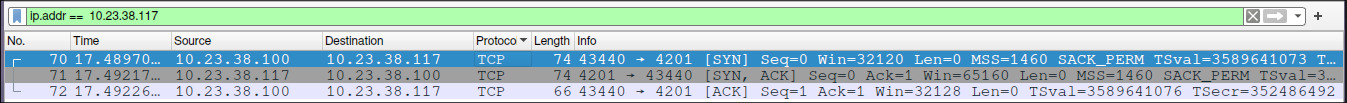
\includegraphics[scale=0.3]{images/handshake.jpeg}
	\caption{TCP 3 Way Handshake}
\end{figure}
\subsubsection{Nachrichten verschicken und empfangen}
\begin{figure}[h]
	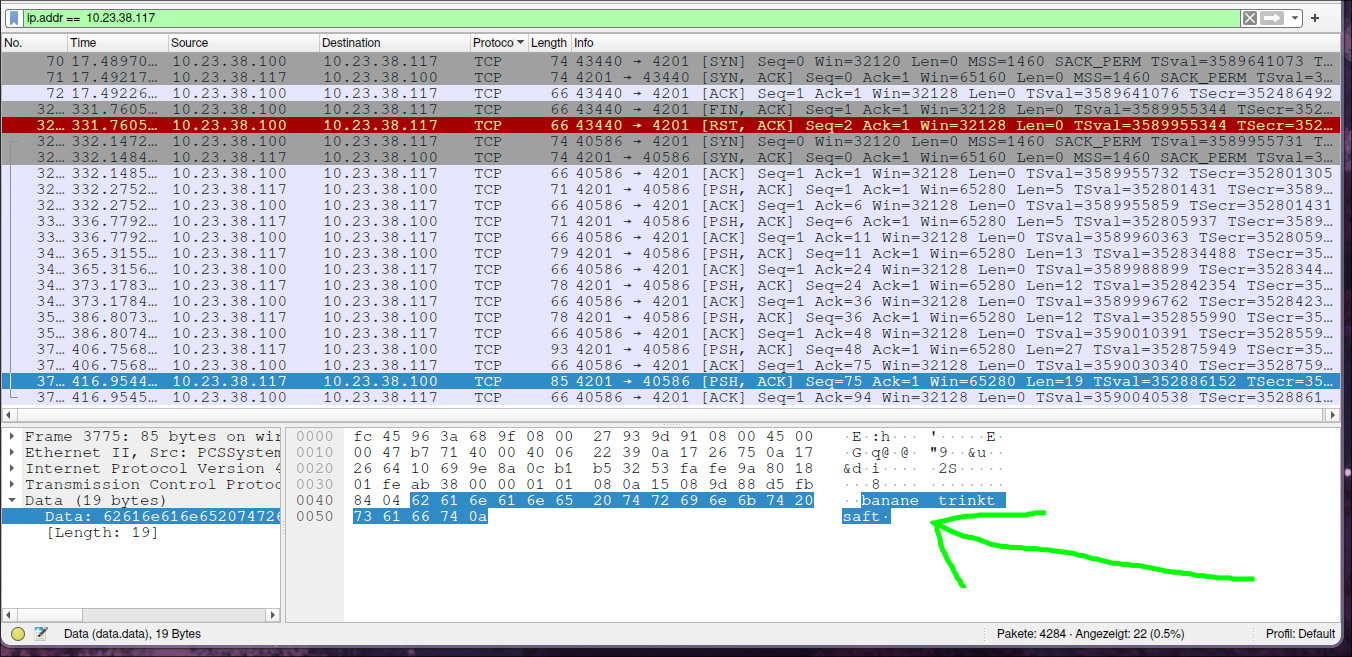
\includegraphics[scale=0.3]{images/nachricht.jpeg}
	\caption{Nachricht}
\end{figure}
\newpage
\subsubsection{TCP-Flags}
% https://www.geeksforgeeks.org/tcp-flags/
% den schaß citen
TCP-Flags dienen dazu um den Zustand, oder andere zusätzliche Informationen der Verbindung anzuzeigen.\\
Diese diesen zum Troubleshooten.
In der Übung ist die Push flag gesetzt, was bedeuted, dass die Nachricht sofort übertragen wird, ohne darauf zu warten, dass zusätliche Informationen auf der Senderseite gebuffert werden.\cite{TCP-Flags}
\\ Wird oft in Echtzeitapplikation benutzt.
\begin{figure}[h]
	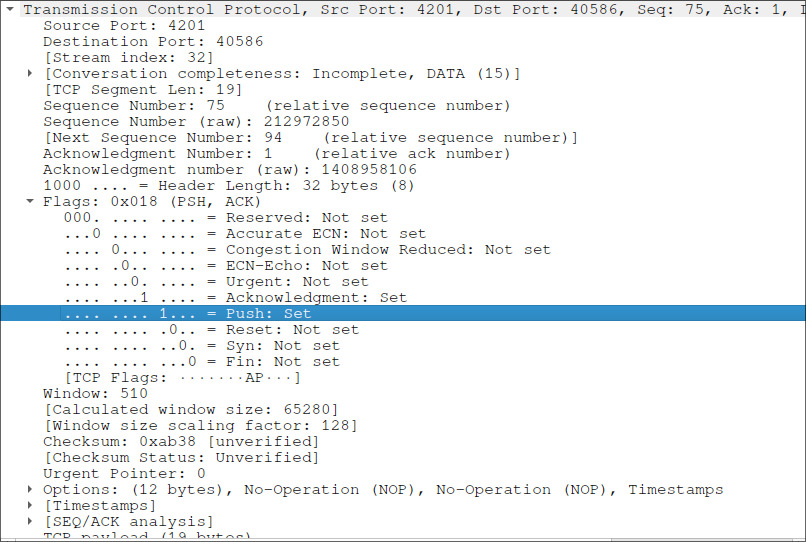
\includegraphics[scale=0.5]{images/tcp-flags.jpeg}
	\caption{TCP-Flags}
\end{figure}
\newpage
\subsubsection{TCP-Header}
%https://networklessons.com/cisco/ccie-routing-switching-written/tcp-header
Vorhandenen Felder
\begin{outline}
	\1 Source Port
	\1 Destination Port
	\1 Sequence Number
	\2 Zeigt an wie viele Daten in der TCP Session übertragen werden.
	\1 Acknowledgment Number
	\2 Vom Empfänger benutzt um das Nächste TCP Segment anzufordern
\end{outline}
Nicht Vorhandene Felder
\begin{outline}
	\1 Window
	\2 Gibt an wie viele bytes die der Empfänger empfangen will. Wird genutzt damit der Empfänger sagen kann, dass er mehr Daten empfagen will.
	\1 RSV
	\2 3 Reservierte Bits, die immer 0 sind.
	\1 Urgent Pointer
	\1 DO
	\2 Länge des Headers.
	\1 Flags
	\2 Vorher bereits erklärt.
	\1 Checksum
	\2 Benutzt für eine Prüfsumme um sicherzugehen, dass der TCP header korrekt is.
\end{outline}
\cite{TCP-Header}
\begin{figure}[h]
	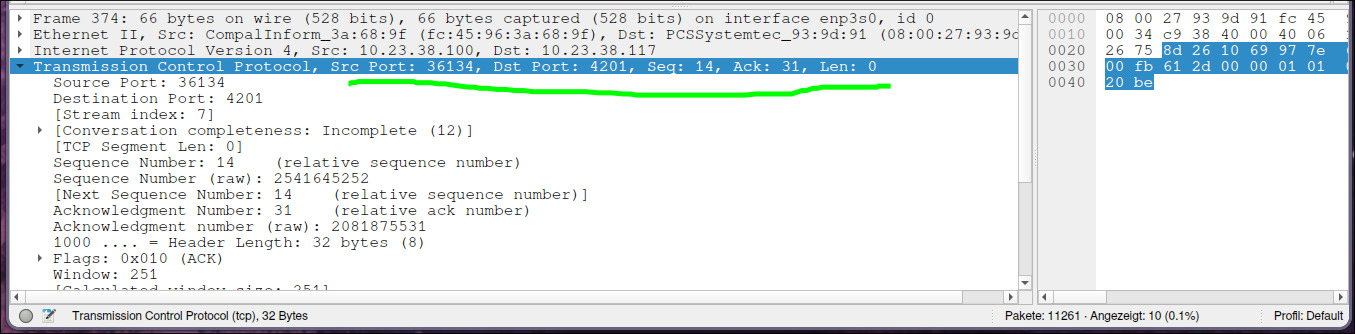
\includegraphics[scale=0.2]{images/tcp-header.jpeg}
	\caption{TCP-Header}
\end{figure}
\newpage
\subsubsection{Verbindungsabbruch}
\begin{figure}[ht]
	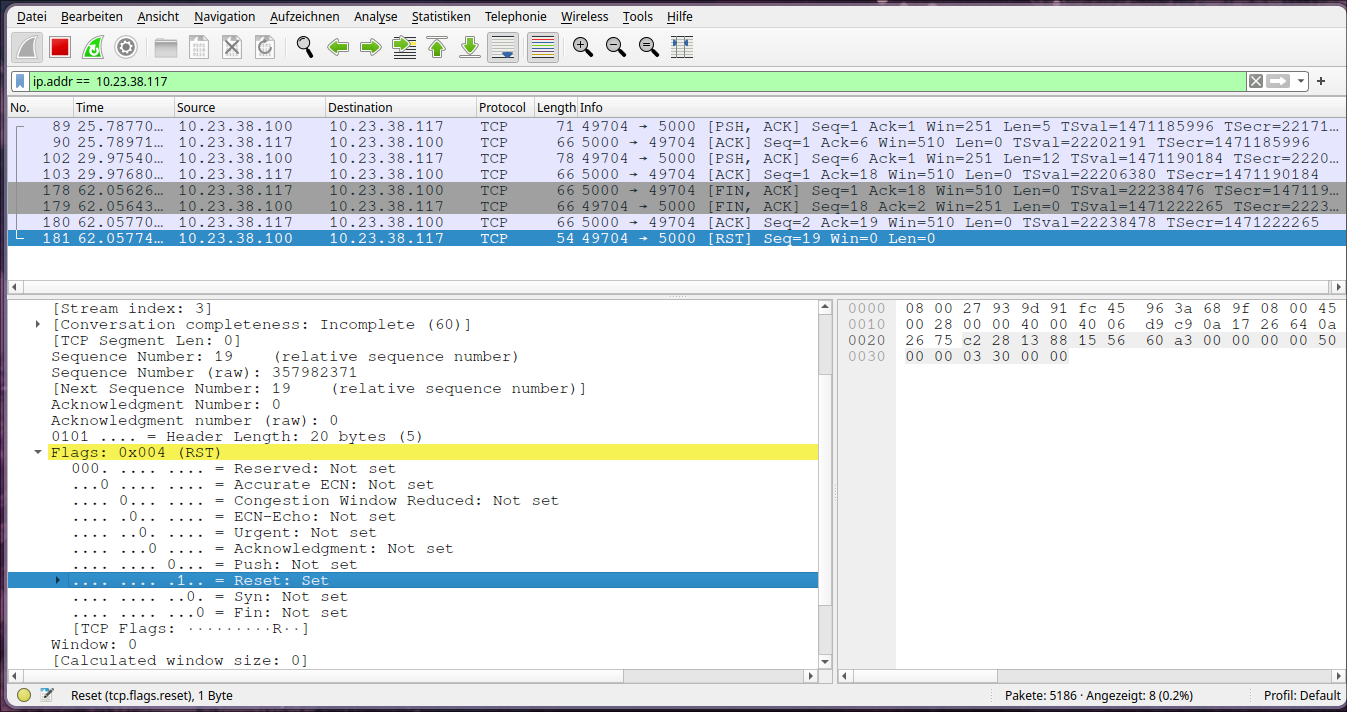
\includegraphics[scale=0.2]{images/verbindungsabbruch.png}
	\caption{Verbindungsabbruch}
\end{figure}

Die TCP-Flag Reset wird im Packet gesetzt und dann ist die Verbindung mit diesem Packet beendet.
\subsubsection{Verbinden mit dem Sever (UDP)}
nc -u 10.23.38.117 4201
\subsubsection{UDP-Verbindungsaufbau}
\begin{figure}[h]
	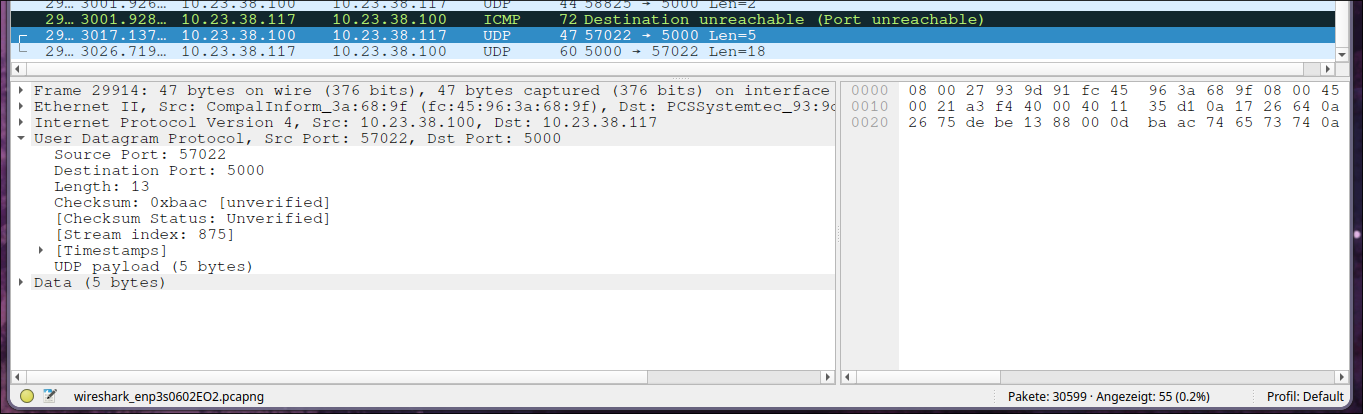
\includegraphics[scale=0.3]{images/udpverbindungsaufbau.png}
	\caption{UDP-Verbindungsaufbau}
\end{figure}

Im gegensatz zu TCP gibt es hier keinen 3-Way-Handsake und die Verbindung beginnt direkt.
\subsubsection{UDP-Nachrichten}
\begin{figure}[h]
	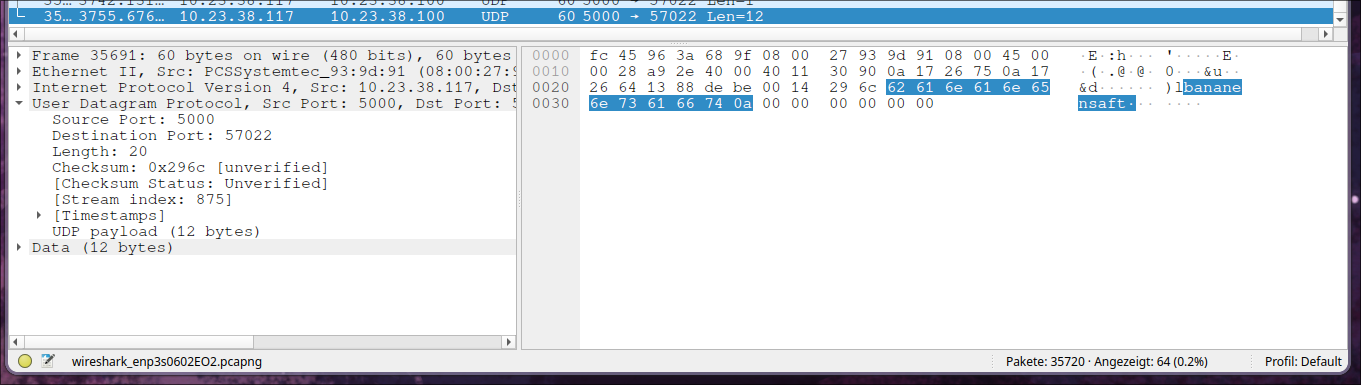
\includegraphics[scale=0.3]{images/udp-nachricht.png}
	\caption{UDP-Nachricht}
\end{figure}
\subsubsection {UDP-Header}
%https://de.wikipedia.org/wiki/User_Datagram_Protocol
\begin{outline}
	\1 Source Port
	\1 Destination Port
	\1 Länge
	\1 Checksum
\end{outline}
Diese Felder haben die selben bedeutungen wie bei TCP.
\cite{UDP}
\subsubsection{UDP-Verbindungsabbruch}
\begin{figure}[h]
	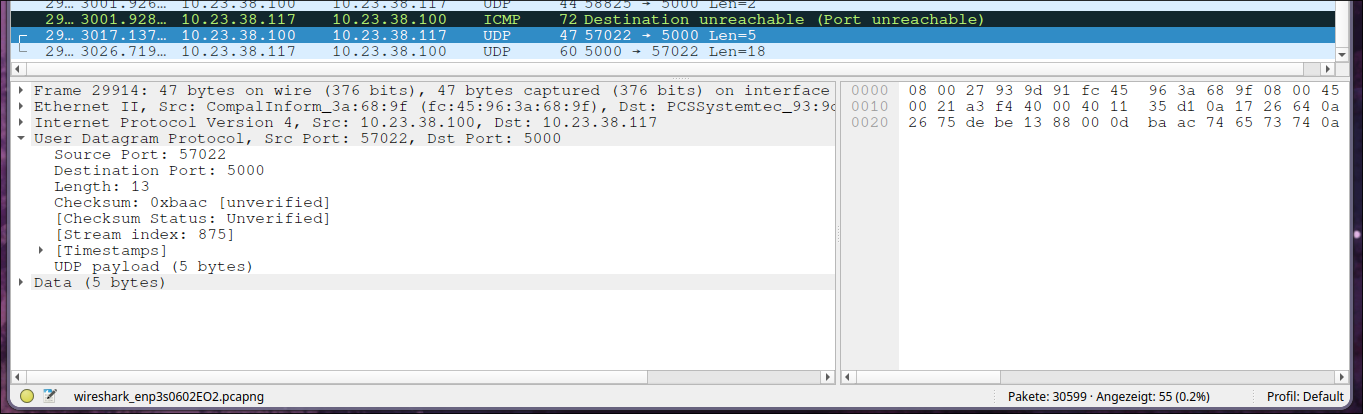
\includegraphics[scale=0.3]{images/udpverbindungsaufbau.png}
	\caption{UDP-Verbindungsabbruch}
\end{figure}
Die Verbindung endet einfach und es wird kein Packet zum Beenden der Verbindung geschickt.
\section{TCP und UDP Headervergleich}



\newpage
\section{Quellen}
\bibliography{quellen}
\newpage
\section{Abbildungsverzeichnis}

\listoffigures

\end{document}
